Questo problema trova quindi una forte applicazione, come già sottolineato, nell'ambito della teoria del controllo: ma quindi, come possiamo applicare tecniche di reinforcement learning per andare a completare questo compito, ovvero quello di cercare di mantenere il pendolo in posizione verticale?

Come ben sappiamo, e come è evidente nel contesto del Cart Pole (figura ~\ref{fig:ActionBehaviour}), si tratta di andare a determinare il corretto input (\textit{azione}) al sistema il quale genererà il comportamento desiderato.

\begin{figure}[!h]
	\centering
	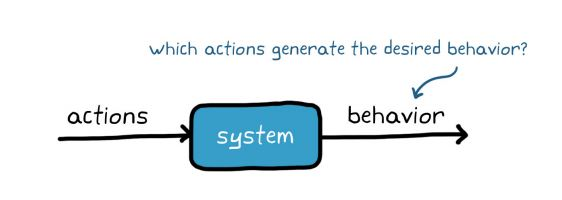
\includegraphics[width=0.4\textwidth]{Immagini/In_Out.JPG}
	\caption{Concetto di input-output}
	\label{fig:ActionBehaviour}
\end{figure}

La scelta dell'azione da portare all'ingresso del sistema, ovvero di quale movimento il carrello deve effettuare, solitamente viene realizzata andando ad utilizzare un sistema di retroazione ad anello chiuso, per cercare così di migliorare le prestazioni, riducendo l'errore (figura ~\ref{fig:ControlTheory})

\begin{figure}[!h]
	\centering
	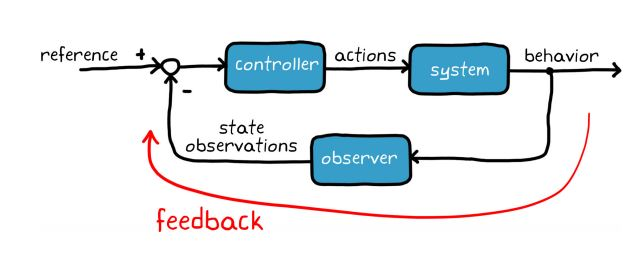
\includegraphics[width=0.6\textwidth]{Immagini/ControlTheory.JPG}
	\caption{Rete di retroazione}
	\label{fig:ControlTheory}
\end{figure}
Questo concetto è semplice da esprimere a parole e a livello grafico, però, nelle applicazioni reali, può diventare estremamente difficile da ottenere, nel momento in cui il sistema è molto complesso da modellizzare matematicamente, oppure presenta forti componenti non lineari, oppure ancora presenta un elevato spazio degli stati.

Ci viene quindi in aiuto, nel contesto del controllo, il reinforcement learning, il quale permette di andare a condensare in un'unica \textit{black-box} tutto il sistema di controllo, andando a ricevere come ingresso l'insieme di tutte le osservazioni dell'ambiente esterno e fornendo come output le azioni dirette (figura ~\ref{fig:SqueezingOfControlTheory})

\begin{figure}[h!]
	\centering
	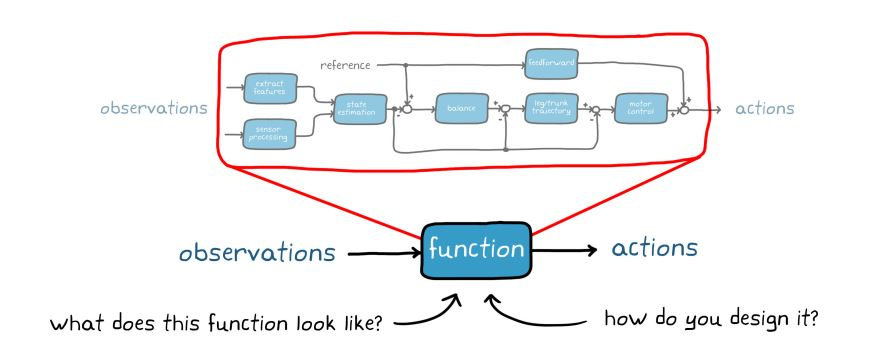
\includegraphics[width=0.8\textwidth]{Immagini/SqueezingOfControlTheory.JPG}
	\caption{Modellizzazione \textit{black - box}}
	\label{fig:SqueezingOfControlTheory}
\end{figure}

La peculiarità dei sistemi di reinforcement learning, a differenza delle altre due branchie del \textit{machine learning} (\textit{supervised learning e unsupervised learning}), sta nel fatto che essi vanno a lavorare con dati provenienti da ambienti dinamici, imponendosi l'obbiettivo di andare a trovare la miglior sequenza di azioni che andrà a generare il miglior \textit{output}, ovvero vale a dire il più alto reward ottenibile dall'agente stesso.

Nel fare questo l'agente risulta essere in grado di osservare lo stato attuale dell'\textit{environment}, decidendo poi quali azioni compiere: ovviamente, andando ad eseguire certe azioni, lo stato dell'ambiente cambia, fornendo un certo \textit{reward} all'agente stesso, in base al quale esso può valutare se l'azione eseguita era "buona" oppure se è meglio evitare di ripeterla (questo ciclo è sinteticamente rappresentato in figura ~\ref{fig:State_Action_Reward}).

\begin{figure}[h]
	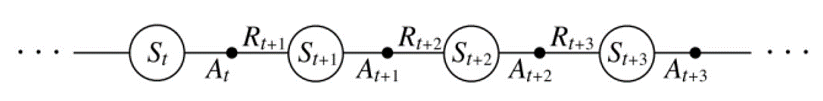
\includegraphics[width=0.7\textwidth]{Immagini/State_Action_Reward.png}
	\caption{Sequenza \textit{State-Action-Reward}}
	\label{fig:State_Action_Reward}
\end{figure}

In particolare, la da parte dell'agente di quale azione eseguire, in seguito a quello che è lo stato osservato, avviene per mezzo di una funzione la quale, nella nomenclatura del RL è chiamata \textit{policy} (figura ~\ref{fig:Policy}).

\begin{figure}[!h]
	\centering
	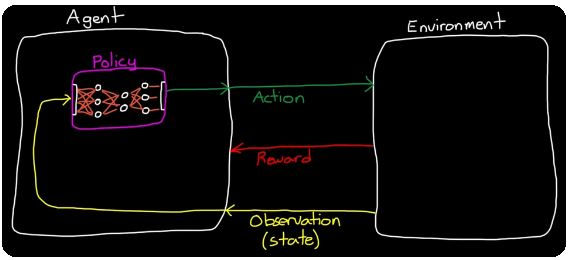
\includegraphics[width=0.7\textwidth]{Immagini/Policy.JPG}
	\caption{Policy}
	\label{fig:Policy}
\end{figure}

Ovviamente questa mappatura \textit{observation (state) - action} non può essere realizzata in maniera statica, anche se trovassimo la miglior policy: questo perchè l'ambiente potrebbe cambiare (e quasi sicuramente lo farà!) nel corso del tempo, e quindi una mappatura statica non sarebbe del tutto ottimale.

Questo quindi porta alla necessità di introdurre \textit{RL alogorithms}, i quali permettono di andare ad aggiornare la policy, in base alla stato-azione-reward, cercando quindi di scegliere la policy ottimale per ogni stato dell'ambiente., ovvero cercando di settare nella maniera migliore i parametri che caratterizzano la funzione espressa, in maniera generica, in figura ~\ref{fig:PolicyFunction}

\begin{figure}[!h]
	\centering
	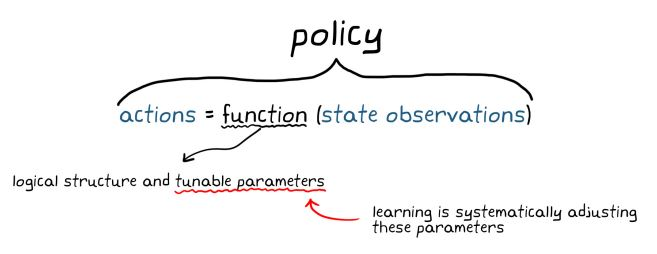
\includegraphics[width=0.5\textwidth]{Immagini/PolicyLearning.JPG}
	\caption{Significato di \textit{imparare} per un agente}
	\label{fig:PolicyFunction}
\end{figure}

\newpage

In sostanza questo update della policy può avvenire seguendo differenti algoritmi, come vedremo successivamente: in ogni caso, indipendentemente dalla strategia che si decide di seguire per scegliere l'azione successiva, possiamo modellizzare questo update come un blocco interno all'agente e che lavora direttamente sulla policy, basandosi sulla condizione attuale dell'ambiente, sull'azione che si va ad eseguire e sul reward che si ottiene eseguendola (il tutto è schemattizzato in figura ~\ref{label})

\begin{figure}[!h]
	\centering
	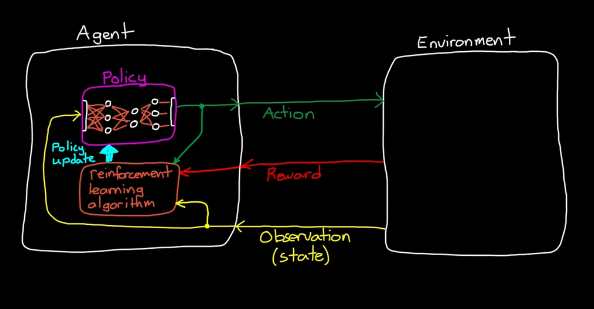
\includegraphics[width=0.5\textwidth]{Immagini/Policy_update.png}
	\caption{Policy update con algoritmi di \textit{RL}}
	\label{fig:Policy_update}
\end{figure}


E' a questo punto che possiamo quindi esplicitare il diretto legame tra RL e control theory: come abbiamo visto con entrambi i metodi vogliamo andare a determinare la corretta azione da eseguire sul sistema, per ottenere il comportamento desiderato, da cui si ricava il feedback, che corrisponde alle osservazioni dello stato del sistema (figura ~\ref{fig:RL_Control}).

\begin{figure}[!h]
	\centering
	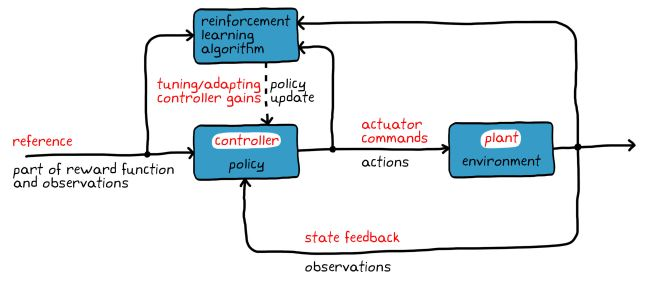
\includegraphics[width=0.7\textwidth]{Immagini/RL_Control.JPG}
	\caption{RL inteso come \textit{control theory}}
	\label{fig:RL_Control}
\end{figure}